\section{A Model}

First, we develop a simple model of posting behavior to ground our empirical work. Then, we test whether the predictions of the model are supported by the data.

\subsection{A model of pay-to-post}

We envision a model in which a user receives ``post ideas'' as a Poisson arrival process with rate $\gamma$. Post ideas arrive with a quality level $q$, which affects how other users respond to the post, and an intrinsic motivation to post it, $\epsilon$. The level of internal motivation may be correlated with post quality, and they are drawn from a joint probability density function $f(q,\epsilon)$. We allow different users to draw from different distributions of $(q,\epsilon)$, but for now we focus on the decisions of a single user.

By Bayes' Rule, $f(q, \epsilon) = f_{\epsilon|q} (\epsilon | q) f_q (q)$, where $f_{\epsilon|q}(\cdot)$ is the conditional density of $\epsilon$ given $q$, and $f_q(\cdot)$ is the marginal density of $q$. We assume that $f_{\epsilon|q}(\cdot)$ is strictly log-concave and weakly satisfies the monotone likelihood ratio property in $\epsilon$ with respect to $q$:

\begin{assumption}[Log Concavity]\label{asm_logconcavity}
For each $q$, $f_{\epsilon|q}(\cdot | q)$ is strictly log-concave; that is, $\ln f_{\epsilon|q} (\epsilon | q)$ is strictly concave in $\epsilon$.
\end{assumption}
\begin{assumption}[Monotone Likelihood Ratio Property]\label{asm_mlrp}
For any $q_2 > q_1$, the likelihood ratio of the conditional densities,
\begin{align*}
\ell(\epsilon;q_1, q_2) = \frac{f_{\epsilon|q}(\epsilon|q_2)}{f_{\epsilon|q}(\epsilon|q_1)}
\end{align*}
is weakly increasing in $\epsilon$.
\end{assumption}
\noindent \emph{Remark.}  Assumption \ref{asm_logconcavity} limits the heaviness of the tail of the motivation distribution. Intuitively, it ensures that the extreme tail of the motivation distribution is not thick enough to swamp quality selection effects at very high posting costs. It is not a strong assumption, and it is satisfied by most commonly used distributional families, including the normal and logistic distributions.\footnote{Weaker, local conditions about the hazard rate in the neighborhood of the current posting cost would also suffice, but we state the stronger condition of global log-concavity for simplicity. Moreover, strict log-concavity is assumed for simplicity, but it suffices to assume either strict log-concavity or strict monotone likelihood ratio property; we do not need strictness for both.}

Assumption \ref{asm_mlrp} is a non-negative dependence condition between post quality $q$ and intrinsic motivation $\epsilon$. Informally, it says that higher quality ideas tend to come with (weakly) higher intrinsic desire to post: when $q$ is higher, the distribution of $\epsilon$ shifts to the right. Independence between $\epsilon$ and $q$ is allowed as a special case, but the assumption rules out systematic negative dependence. In our context, this means that users who receive a high quality post idea are also (weakly) more likely to feel a strong intrinsic desire to post it. As we shall document later, this is consistent with users' self reported perceptions of their own motivations. \hfill \qedsymbol

~

\noindent Once a post is made, zaps arrive according to a Poisson process. Both the arrival rate of zaps and the amount of each zap are dependent on the quality of the post, $q$. Let $\lambda(q)$ be the arrival rate as a function of $q$, and let $E[z|q]$ be the expected zap amount per zap conditional on $q$. 

Supposing the user has a discount factor of $\rho$, the expected present value of the Poisson stream of zaps is equal to:\footnote{This follows from $V(q) = \int_{0}^{\infty} e^{-\rho t} \lambda(q) E[z|q] dt$.}
\begin{align}
V(q) = \frac{\lambda(q)}{\rho} E \left[z | q\right] \label{eq_V}
\end{align}
We assume that $V(q)$ is continuous and strictly increasing in $q$, which merely says that the expected present value of zaps is higher for higher quality posts:

\begin{assumption}[Monotone Returns to Quality]\label{asm_monotonicity}
$V(q) = \frac{\lambda(q)}{\rho} E[z|q]$ is continuous and strictly increasing in $q$.
\end{assumption}

~

\noindent  The user will make the post if their expected present value of zaps plus their intrinsic motivation is greater than the posting cost $c$:
\begin{align}
\text{Post} = 1 \text{ if } V(q) + \epsilon > c \text{ and } 0 \text{ otherwise }
\end{align}
From the perspective of the user, $c$ is fixed and known at the time of the post.

We now demonstrate conditions under which an increase in posting cost $c$ will lead to fewer posts, but higher quality posts.

\begin{proposition} \label{prop_pay_to_post}
Suppose Assumptions \ref{asm_logconcavity}-\ref{asm_monotonicity} hold. Then an increase in $c$:
\begin{enumerate}[label=(\roman*)]
\item strictly decreases the probability that the post idea is posted, and
\item strictly increases the expected quality of posts, conditional on posting.
\end{enumerate}
\end{proposition}

\begin{proof}
A proof is provided in the appendix.
\end{proof}

\noindent \emph{Remark.} Proposition \ref{prop_pay_to_post} implies that when posting cost increases, users are less likely to post, but that when they do post, the average quality of the post is higher. Although the proposition is stated from the perspective of a single user, we note that as long as the global joint distribution of $(q,\epsilon)$ holds to Assumptions \ref{asm_logconcavity} and \ref{asm_mlrp}, and if Assumption \ref{asm_monotonicity} also holds for all users, then Proposition \ref{prop_pay_to_post} applies in the aggregate, even if users have heterogeneous marginal densities for $q$ and $\epsilon$. 

The result of Proposition \ref{prop_pay_to_post} extends to a setting with multiple territories. Users post in the territory $j$ that maximizes $V_j(q_j) + \epsilon_j - c_j$, provided it is positive. When territory $j$ raises its posting cost $c_j$, users' outside options are unaffected, so the same logic applies: as long as the population-level joint distribution of quality and motivation within each territory satisfies Assumptions \ref{asm_logconcavity}-\ref{asm_monotonicity}, a territory that raises its posting cost will see fewer but higher quality posts. \hfill \qedsymbol




\subsubsection*{Proof of Proposition \ref{prop_pay_to_post}}

\begin{proof}
A post idea $(q, \epsilon)$ is posted if and only if $\epsilon > c - V(q)$. Define $\pi(q,c)$ as the probability (over $\epsilon$) that a post of quality is posted when the cost is $c$:
\begin{align*}
\pi(q,c) &= P(\epsilon > c - V(q)) 
\end{align*}
$\pi(q,c)$ is equivalent to the survival function of $\epsilon|q$, evaluated at $c - V(q)$: $\pi(q,c) = S_{\epsilon|q}(c - V(q) | q)$.
\begin{enumerate}[label=(\roman*)]
\item The unconditional probability of posting is:
\begin{align*}
P(\text{post}) = \int S_{\epsilon|q}(c-V(q)|q)f_q(q)dq
\end{align*}
Since $S_{\epsilon|q}(\cdot|q)$ is a survival function, its first derivative is negative everywhere. An increase in $c$ will therefore reduce the value of $S_{\epsilon|q}(c - V(q))$ at every $q$. Since that is what we are integrating over to get $P(\text{post})$, this strictly reduces $P(\text{post})$. The expected number of posts per unit time is $\gamma P(\text{post})$, so an increase in $c$ strictly reduces the expected number of posts.

\item Take any $c^\prime > c$. The set of ideas that were posted at cost $c$ can be partitioned into two groups:
\begin{itemize}
\item \textbf{Surviving posts.} Ideas that are still posted at cost $c^\prime$, i.e. $V(q) + \epsilon > c^\prime$
\item \textbf{Marginal posts.} Ideas that are posted at $c$ but not at $c^\prime$, i.e. $c < V(q) + \epsilon < c^\prime$.
\end{itemize}
By the Law of Iterated Expectations,
\begin{align*}
E[q | \text{post at } c] = \alpha E[q | \text{surviving}] + (1-\alpha) E[q | \text{marginal}]
\end{align*}
where $\alpha = P(\text{surviving} | \text{post at } c)$. Noting that $E[q|\text{post at } c^\prime] = E[q|\text{surviving}]$, we rearrange the above equation to obtain:
\begin{align*}
E[q|\text{post at } c^\prime] - E[q|\text{post at } c] = (1-\alpha) \left( E[q|\text{surviving}] - E[q|\text{marginal}\right)
\end{align*}
Thus, to show that expected post quality is increasing in $c$, it suffices to show that the expected quality of the surviving posts is always higher than the expected quality of the marginal posts. 

To demonstrate this, it is sufficient to establish that for any $q_2 > q_1$, the ratio $\pi(q_2,c)/\pi(q_1,c)$ is strictly increasing in $c$. Intuitively, this says that as costs rise, higher quality posts retain a larger share of the posting probability relative to lower quality ideas. This would imply that the marginal posts are tilted towards lower quality than surviving posts.

We write:
\begin{align*}
\frac{\pi(q_2,c)}{\pi(q_1,c)} = \frac{S_{\epsilon|q}(c-V(q_2)|q_2)}{S_{\epsilon|q}(c-V(q_1)|q_1)} \label{eq_prob_ratio}
\end{align*}
Define the hazard rate: $h(\epsilon|q) = f_{\epsilon|q}(\epsilon|q) / S_{\epsilon|q}(\epsilon|q)$. Differentiating $\pi(q_2,c)/\pi(q_1,c)$ with respect to $c$ shows us that the ratio is increasing in $c$ if and only if:
\begin{align*}
h(c - V(q_1) | q_1) > h(c - V(q_2) | q_2)
\end{align*}
The proof now proceeds in two parts. 

\paragraph{Claim 1.} First, we show that $h(\epsilon | q_1) \geq h(\epsilon | q_2)$ for any $q_2 > q_1$. By the MLRP, for any $t > \epsilon$, we have that $\ell(t; q_1, q_2) \geq \ell(\epsilon; q_1, q_2)$, which rearranges to:
\begin{align*}
f_{\epsilon|q}(t|q_2) f_{\epsilon|q}(\epsilon|q_1) \geq f_{\epsilon|q}(\epsilon|q_2) f_{\epsilon|q}(t|q_1)
\end{align*}
Integrating both sides over $t$ from $\epsilon$ to $\infty$ gives us:
\begin{align*}
S_{\epsilon|q}(\epsilon|q_2) f_{\epsilon|q}(\epsilon|q_1) \geq S_{\epsilon|q}(\epsilon|q_1) f_{\epsilon|q}(\epsilon|q_2)
\end{align*}
which rearranges to $h(\epsilon|q_1) \geq h(\epsilon | q_2)$ as was to be demonstrated.

\paragraph{Claim 2.} Now, we show that $h(\epsilon|q)$ is increasing in $\epsilon$ for each $q$. Take the derivative of $h(\epsilon|q)$ with respect to $\epsilon$. The sign is equal to the sign of:
\begin{align*}
f_{\epsilon|q}(\epsilon|q)^2 + f^\prime_{\epsilon|q}(\epsilon|q) S_{\epsilon|q}(\epsilon|q)
\end{align*}
When $f^\prime_{\epsilon|q}(\epsilon|q) \geq 0$, this is immediately positive. When $f_{\epsilon|q}^\prime(\epsilon|q)<0$, we rely on the log-concavity property. Since $f_{\epsilon|q}(\cdot)$ is log-concave, the following holds for every $t > \epsilon$:
\begin{align*}
\ln f_{\epsilon|q} (t|q) < \ln f_{\epsilon|q}(\epsilon|q) + (t-\epsilon) \frac{f_{\epsilon|q}^\prime(\epsilon|q)}{f_{\epsilon|q}(\epsilon|q)}
\end{align*}
Exponentiating both sides:
\begin{align*}
f_{\epsilon|q} (t|q) < f_{\epsilon|q}(\epsilon|q) \exp\left[ (t-\epsilon) \frac{f_{\epsilon|q}^\prime(\epsilon|q)}{f_{\epsilon|q}(\epsilon|q)} \right]
\end{align*}
Now integrating over $t$ from $\epsilon$ to $\infty$:
\begin{align*}
S_{\epsilon|q} (\epsilon | q) &< f_{\epsilon|q}(\epsilon|q) \int_{\epsilon}^\infty \exp\left[ (t-\epsilon) \frac{f_{\epsilon|q}^\prime(\epsilon|q)}{f_{\epsilon|q}(\epsilon|q)} \right] dt \\
& = - \frac{f_{\epsilon|q}(\epsilon|q)^2}{f^\prime_{\epsilon|q}(\epsilon|q)}
\end{align*}
Since $f^\prime_{\epsilon|q}(\epsilon|q) < 0$, this can be rearranged to:
\begin{align*}
f_{\epsilon|q}(\epsilon|q)^2 + f^\prime_{\epsilon|q}(\epsilon|q) S_{\epsilon|q}(\epsilon|q) > 0
\end{align*}
which was to be demonstrated. Thus, $h(\epsilon|q)$ is strictly increasing in $\epsilon$ for all $q$.

By the monotonicity assumption, $c - V(q_1) > c - V(q_2)$. By Claim 2, this implies that $h(c - V(q_1)|q_1) > h(c-V(q_2)|q_1)$. By Claim 1, $h(c-V(q_2) | q_1) \geq h(c-V(q_2) | q_2)$. Together, we have $h(c - V(q_1)|q_1) > h(c-V(q_2)|q_2)$, which was to be demonstrated. 
\end{enumerate}
\end{proof}


\subsubsection*{Proof of Proposition \ref{prop_v4v}}

\begin{proof}
Given $\hat{\theta}$, the user's expected utility from effort is:
\begin{align*}
U(e;\hat{\theta}) = E_{q,\epsilon|e} \left[ \max \left\{ \exp (\hat{\theta} + q) - c + \epsilon, 0 \right\} \right] - \kappa(e)
\end{align*}
It suffices to show that $U(e; \hat{\theta})$ is supermodular in $(e, \hat{\theta})$. For any $\hat{\theta}_2 > \hat{\theta}_1$:
\begin{align*}
U(e;&\hat{\theta}_2) - U(e;\hat{\theta}_1) = \\
& E_{q,\epsilon|e}\left[ \max \left\{ \exp( \hat{\theta}_2 + q) - c + \epsilon, 0\right\} - \max \left\{ \exp( \hat{\theta}_1 + q) - c + \epsilon, 0 \right\} \right]
\end{align*}
The integrand is supermodular in $(\hat{\theta},q)$ because  $\exp(\hat{\theta} + q)$ is supermodular in $(\hat{\theta}, q)$ and because the $\max$ operator is convex and increasing. Furthermore, since $F(q|\epsilon;e)$ satisfies FOSD in $e$, it follows immediately $U(e;\hat{\theta}_2)-U(e;\hat{\theta}_1)$ is increasing in $e$, and hence $U(e;\hat{\theta})$ is supermodular in $(e,\hat{\theta}).$
\end{proof}

\section{Methodological Detail - Text Embeddings}

Text embeddings were computed for each post by inputting the post text into \mbox{OpenAI's} \texttt{text-embedding-3-small} embedding model. The embedding model computes a 1,536 dimensional embedding vector for each post that encodes the meaning of the text in such a way that two posts with similar text will have a small distance between their embedding vectors. The raw embedding dimensions are learned from a large general purpose training corpus and are not tailored to the structure of our dataset. We therefore compute the principal components of the raw embedding vectors using our corpus. The principal components are orthogonal linear combinations of the original 1,536 embedding dimensions that explain the greatest variation across posts in our data. Figure \ref{fig_text_scree_plot} shows the scree plot of the principal components analysis, for the first \gn{NumPCAComponentsShow} components. To keep our regression in \eqref{eq_zreg} parsimonious, we decided to use only the first \gn{TextPCAK} components in the analysis. These components explain  \gn{TextPCAPctExplained}\% of the total variation,  but our results in Section \ref{sec_v4v} are robust to the specific choice of how many components to use. After running regression \eqref{eq_zreg}, we inspected the embedding dimensions that were most predictive of zaps. The first most predictive dimension appears to capture meta-posts (not necessarily in the \texttt{meta} territory) about Stacker News itself, such as tips for how to post and earn more sats. The second most predictive dimension appears to capture posts about geopolitical and macroeconomic events, such as a personal discussion about elections in Venezuela. The third dimension most predictive dimension appears to capture posts that ask questions about personal finance. We note that, although these embedding dimensions are the most strongly associated with zaps, other predictive aspects of the text content may not align with any single dimension and may instead be captured by combinations of dimensions. We therefore treat the embedding components primarily as control variables in the regression and avoid over-interpreting individual coefficients or assigning strong substantive meaning to any single dimension.

\pagebreak

\begin{figure}[H]
\caption{Scree Plot for Post Text Embeddings}
\label{fig_text_scree_plot}
\vspace{-0.6cm}
\begin{center}
\begin{adjustbox}{width=\textwidth}
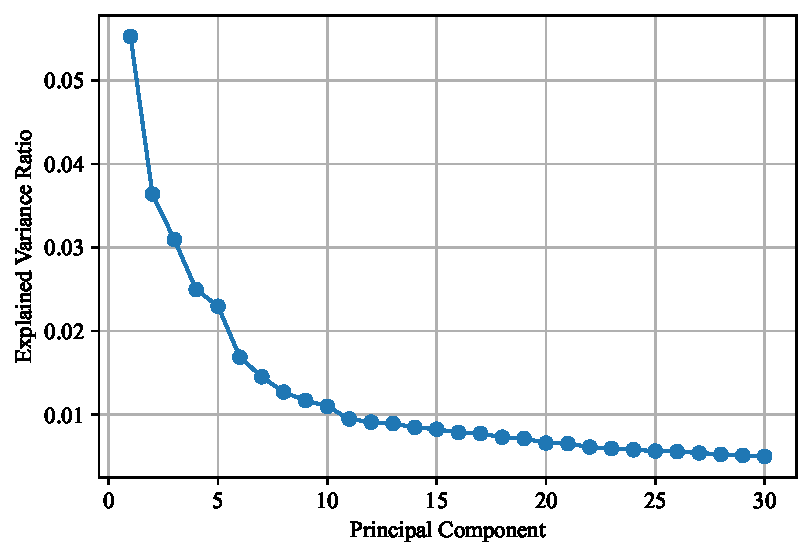
\includegraphics{results/fig_text_scree_plot.pdf}
\end{adjustbox}
\end{center}
\footnotesize \textit{Note:} Shows the scree plot for post text embeddings, indicating the explained variance ratio for each principal component. 
The total explained variance at $K=10$ is \gn{TextPCAPctExplained}\%.
\end{figure}

